\documentclass[11pt,a4paper,spanish]{book}
\usepackage{estilo_unir-1}
\hypersetup{
	colorlinks   = true,
	urlcolor     = blue,
	linkcolor    = black,
	citecolor    = red
}
\usepackage[nottoc]{tocbibind}
\usepackage{tikz}
\usetikzlibrary{arrows.meta, positioning, fit, calc}
\usepackage{listings}
\usepackage{graphicx}
\usepackage{longtable}
\usepackage{booktabs}
\usepackage{multirow}
\lstset{
	basicstyle=\ttfamily\footnotesize,
	breaklines=true,
	frame=single,
	backgroundcolor=\color[gray]{0.95},
	numbers=left,
	numberstyle=\tiny\color[gray]{0.5},
	keywordstyle=\color{blue},
	commentstyle=\color[gray]{0.5},
	tabsize=2
}

%---------------------------
% Datos del trabajo
%---------------------------
\subject{Pr\'{a}cticas Acad\'{e}micas Externas}
\title{Sistema de medici\'{o}n de impedancia (EIS) para cuantificaci\'{o}n de Candida albicans --- Memoria Final}
\author{Andr\'{e}s Alexandro Tapia Flores}
\profesor{Universidad Internacional de la Rioja (UNIR)}
\date{Mayo 2026}

\begin{document}
\renewcommand{\listfigurename}{\'{I}ndice de figuras}
\renewcommand{\listtablename}{\'{I}ndice de tablas}
\renewcommand{\contentsname}{\'{I}ndice de contenidos}
\renewcommand{\figurename}{Figura}
\renewcommand{\tablename}{Tabla}
\setlength{\headheight}{26pt}

\maketitle
\frontmatter
\tableofcontents
\listoffigures
\listoftables

\chapter{Resumen}

Este documento constituye la memoria final del proyecto de desarrollo de un sistema de medici\'{o}n de impedancia electroqu\'{i}mica (EIS) orientado a la cuantificaci\'{o}n de \textit{Candida albicans} en muestras de saliva. El trabajo se enmarca dentro del M\'{a}ster de Computaci\'{o}n Cu\'{a}ntica de la Universidad Internacional de la Rioja (UNIR) y se desarrolla como pr\'{a}cticas acad\'{e}micas externas.

El sistema implementado abarca desde la especificaci\'{o}n de requerimientos hasta la entrega de un producto funcional con arquitectura hardware--software completa. La capa f\'{i}sica se basa en el microcontrolador ESP32 y el analizador de impedancia AD5933, mientras que el software se implementa enteramente en Python con un frontend en React. Debido a la indisponibilidad temporal del equipo de laboratorio, la validaci\'{o}n se realiza mediante una tarjeta de adquisici\'{o}n simulada que preserva el contrato de comunicaci\'{o}n serial del firmware original.

Los aportes principales del trabajo son: (1) un protocolo de comunicaci\'{o}n robusto entre Python y ESP32 mediante comandos de texto y respuestas JSON; (2) un backend as\'{i}ncrono con servidor WebSocket para distribuci\'{o}n en tiempo real; (3) una interfaz web interactiva con visualizaci\'{o}n de diagramas de Bode y Nyquist; (4) un modelo de sesi\'{o}n con persistencia multi--formato (CSV, JSON, resumen textual); (5) un clasificador cu\'{a}ntico variacional simulado de 4 qubits con comparador cl\'{a}sico integrado; y (6) un manual de usuario y reporte t\'{e}cnico que documentan el sistema para su uso y mantenimiento.

El cap\'{i}tulo~5 presenta una secci\'{o}n espec\'{i}fica de computaci\'{o}n cu\'{a}ntica aplicada, detallando la arquitectura del clasificador variacional, el enfoque h\'{i}brido cu\'{a}ntico-cl\'{a}sico, la comparaci\'{o}n de rendimiento entre ambos paradigmas y la evaluaci\'{o}n de impacto en la clasificaci\'{o}n de espectros EIS.

\vspace{0.5cm}
{\bf Palabras clave:} espectroscop\'{i}a de impedancia electroqu\'{i}mica, candida albicans, clasificaci\'{o}n cu\'{a}ntica, circuito variacional cu\'{a}ntico, esp32, ad5933, interfaz web, python, memoria final

\chapter{Abstract}

This document presents the final report of the development of an electrochemical impedance spectroscopy (EIS) measurement system aimed at the quantification of \textit{Candida albicans} in saliva samples. The work is framed within the Master's Degree in Quantum Computing at Universidad Internacional de la Rioja (UNIR) and is developed as external academic internships.

The implemented system spans from requirements specification to the delivery of a functional product with a complete hardware--software architecture. The physical layer is based on the ESP32 microcontroller and the AD5933 impedance analyzer, while the software is entirely implemented in Python with a React frontend. Due to temporary unavailability of laboratory equipment, validation is performed using a simulated acquisition board that preserves the serial communication contract of the original firmware.

The main contributions are: (1) a robust communication protocol between Python and ESP32 using text commands and JSON responses; (2) an asynchronous backend with WebSocket server for real--time distribution; (3) an interactive web interface with Bode and Nyquist diagram visualization; (4) a session model with multi--format persistence (CSV, JSON, textual summary); (5) a simulated 4--qubit variational quantum classifier with integrated classical comparator; and (6) a user manual and technical report documenting the system for use and maintenance.

Chapter~5 provides a dedicated section on applied quantum computing, detailing the variational classifier architecture, the hybrid quantum-classical approach, comparative performance analysis between both paradigms, and the impact assessment on EIS spectrum classification.

\vspace{0.5cm}
{\bf Keywords:} electrochemical impedance spectroscopy, candida albicans, quantum classification, variational quantum circuit, esp32, ad5933, web interface, python, final report

\mainmatter

%=======================================================================
% CHAPTER 1: INTRODUCCION
%=======================================================================
\chapter{Introducci\'{o}n}

\section{Motivaci\'{o}n y contexto}

La detecci\'{o}n r\'{a}pida y no invasiva de pat\'{o}genos en muestras biol\'{o}gicas es un \'{a}rea de investigaci\'{o}n con alto impacto en salud p\'{u}blica. \textit{Candida albicans} es un hongo oportunista presente en la flora microbiana humana que, bajo ciertas condiciones, puede desencadenar infecciones sist\'{e}micas especialmente peligrosas para pacientes inmunocomprometidos. La espectroscop\'{i}a de impedancia electroqu\'{i}mica (EIS) permite caracterizar propiedades el\'{e}ctricas de interfaces biol\'{o}gicas sin requerir marcadores qu\'{i}micos, lo que la convierte en una t\'{e}cnica atractiva para el desarrollo de biosensores port\'{a}tiles.

Desde la perspectiva de la computaci\'{o}n cu\'{a}ntica, los clasificadores basados en circuitos variacionales ofrecen la posibilidad de explotar espacios de Hilbert exponencialmente grandes para encontrar fronteras de decisi\'{o}n en datos de alta dimensionalidad, como los espectros EIS. Aunque el trabajo no ejecuta circuitos en hardware cu\'{a}ntico real, implementa un simulador vectorial de estado que reproduce fielmente las operaciones de un variational quantum classifier (VQC), permitiendo evaluar la viabilidad del enfoque cu\'{a}ntico en este dominio aplicado.

\section{Planteamiento del Trabajo}

El objetivo del Trabajo es dise\~{n}ar, implementar y documentar un sistema completo de adquisici\'{o}n y an\'{a}lisis de datos EIS para la detecci\'{o}n de \textit{Candida albicans}. El sistema debe:
\begin{itemize}
	\item Controlar un analizador de impedancia AD5933 mediante un microcontrolador ESP32.
	\item Comunicar el hardware con un backend Python a trav\'{e}s de un protocolo serial robusto.
	\item Distribuir datos en tiempo real a una interfaz web mediante WebSocket.
	\item Visualizar espectros de impedancia en diagramas de Bode y Nyquist.
	\item Clasificar muestras mediante un algoritmo cu\'{a}ntico variacional con comparaci\'{o}n cl\'{a}sica.
	\item Persistir sesiones de adquisici\'{o}n con metadatos y exportar en m\'{u}ltiples formatos.
\end{itemize}

La implementaci\'{o}n se realiza en Python puro (sin LabVIEW, que era el entorno originalmente propuesto), lo que facilita la integraci\'{o}n con bibliotecas de an\'{a}lisis de datos y frameworks de computaci\'{o}n cu\'{a}ntica.

\section{Estructura del Trabajo}

La memoria se organiza en los siguientes cap\'{i}tulos:
\begin{itemize}
	\item Cap\'{i}tulo~2: Objetivos generales y espec\'{i}ficos del proyecto.
	\item Cap\'{i}tulo~3: Arquitectura del sistema, describiendo las tres capas (hardware, backend, frontend).
	\item Cap\'{i}tulo~4: Desarrollo t\'{e}cnico, detallando las cuatro fases de implementaci\'{o}n.
	\item Cap\'{i}tulo~5: Computaci\'{o}n cu\'{a}ntica aplicada, con la arquitectura VQC, el enfoque h\'{i}brido, comparaci\'{o}n de resultados y evaluaci\'{o}n de impacto.
	\item Cap\'{i}tulo~6: Validaci\'{o}n y resultados, incluyendo an\'{a}lisis de repetibilidad, cargas patr\'{o}n y sensibilidad a efectos electromagn\'{e}ticos.
	\item Cap\'{i}tulo~7: Conclusiones y l\'{i}neas de trabajo futuro.
\end{itemize}

\noindent El manual de usuario se presenta como documento separado (\textit{fase5\_manual\_usuario.pdf}) con gu\'{i}as de instalaci\'{o}n, operaci\'{o}n, interpretaci\'{o}n de resultados y resoluci\'{o}n de problemas.

%=======================================================================
% CHAPTER 2: OBJETIVOS
%=======================================================================
\chapter{Objetivos}

\section{Objetivo general}

Dise\~{n}ar, implementar y validar un sistema de medici\'{o}n de impedancia electroqu\'{i}mica (EIS) basado en ESP32 y AD5933, con backend en Python, interfaz web en React, clasificador cu\'{a}ntico variacional simulado y subsistema de persistencia multi--formato, orientado a la cuantificaci\'{o}n de \textit{Candida albicans} en muestras de saliva.

\section{Objetivos espec\'{i}ficos}

\begin{enumerate}
	\item Especificar los requerimientos funcionales del sistema y definir su arquitectura de bloques.
	\item Implementar un protocolo de comunicaci\'{o}n bidireccional Python--ESP32 sobre puerto serial con formato JSON.
	\item Desarrollar un backend as\'{i}ncrono que consuma datos del hardware, los distribuya por WebSocket y gestione sesiones de adquisici\'{o}n.
	\item Construir una interfaz web interactiva que visualice en tiempo real diagramas de Bode (magnitud y fase) y Nyquist.
	\item Implementar un clasificador cu\'{a}ntico variacional simulado de 4 qubits con codificaci\'{o}n angular y ansatz parametrizado.
	\item Desarrollar un comparador cl\'{a}sico de referencia para evaluar la salida del clasificador cu\'{a}ntico.
	\item Dise\~{n}ar un modelo de sesi\'{o}n persistente que almacene metadatos, eventos y datos en CSV, JSON y resumen textual.
	\item Documentar el sistema mediante un reporte t\'{e}cnico y un manual de usuario completos.
	\item Validar el sistema con an\'{a}lisis de repetibilidad, cargas patr\'{o}n y soluciones control.
\end{enumerate}

%=======================================================================
% CHAPTER 3: ARQUITECTURA DEL SISTEMA
%=======================================================================
\chapter{Arquitectura del sistema}

\section{Dise\~{n}o general}

El sistema se estructura en tres capas principales: hardware de medici\'{o}n, backend de comunicaci\'{o}n y procesamiento, y frontend de visualizaci\'{o}n e interacci\'{o}n. La Figura~\ref{fig:arquitectura-general} presenta el diagrama de bloques completo.

\begin{figure}[ht]
\centering
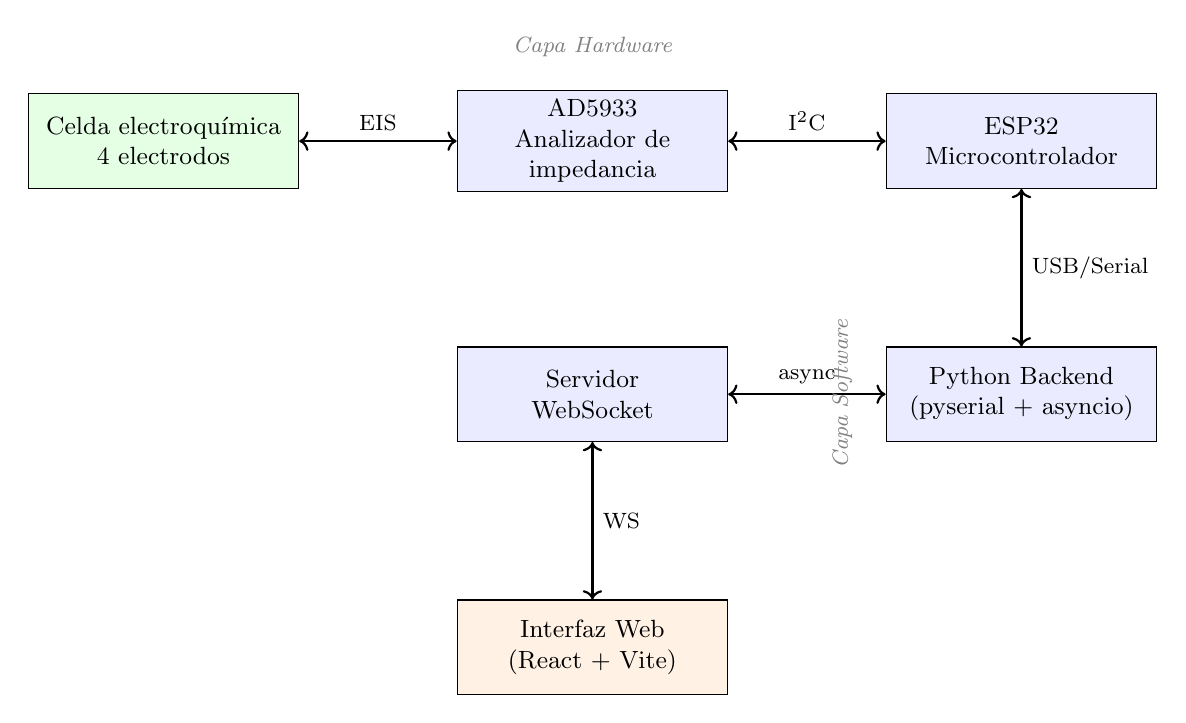
\begin{tikzpicture}[
	block/.style={rectangle, draw, fill=blue!8, text width=3.2cm, minimum height=1.2cm, align=center, font=\small},
	arrow/.style={-{Stealth[length=3mm]}, thick},
	node distance=1.5cm and 2cm
]
	% Hardware layer
	\node[block, fill=green!10] (cell) {Celda electroqu\'{i}mica\\4 electrodos};
	\node[block, right=of cell] (ad5933) {AD5933\\Analizador de\\impedancia};
	\node[block, right=of ad5933] (esp32) {ESP32\\Microcontrolador};

	% Software layer
	\node[block, below=2cm of esp32] (python) {Python Backend\\(pyserial + asyncio)};
	\node[block, left=of python] (ws) {Servidor\\WebSocket};

	% Frontend
	\node[block, below=2cm of ws, fill=orange!10] (web) {Interfaz Web\\(React + Vite)};

	% Arrows
	\draw[arrow, <->] (cell) -- node[above, font=\footnotesize]{EIS} (ad5933);
	\draw[arrow, <->] (ad5933) -- node[above, font=\footnotesize]{I\textsuperscript{2}C} (esp32);
	\draw[arrow, <->] (esp32) -- node[right, font=\footnotesize]{USB/Serial} (python);
	\draw[arrow, <->] (python) -- node[above, font=\footnotesize]{async} (ws);
	\draw[arrow, <->] (ws) -- node[right, font=\footnotesize]{WS} (web);

	% Labels
	\node[above=0.3cm of ad5933, font=\footnotesize\itshape, text=gray] {Capa Hardware};
	\node[left=0.3cm of python, font=\footnotesize\itshape, text=gray, rotate=90, anchor=south] {Capa Software};
\end{tikzpicture}
\caption[Arquitectura general del sistema]{Arquitectura del sistema EIS completo. Fuente: elaboraci\'{o}n propia.}
\label{fig:arquitectura-general}
\end{figure}

\section{Capa hardware}

\subsection{Celda electroqu\'{i}mica}

La celda consta de cuatro electrodos dispuestos para medir impedancia de manera precisa, separando el circuito de excitaci\'{o}n del de medici\'{o}n. El volumen de muestra es de 1~mL de saliva. La presencia de biopel\'{i}cula de \textit{Candida albicans} modifica la impedancia de la interfaz electroqu\'{i}mica, lo que permite distinguir muestras positivas de controles negativos.

\subsection{AD5940 / AD5933}

La especificaci\'{o}n original del proyecto contempla la tarjeta de evaluaci\'{o}n EVAL-AD5940ELCZ de Analog Devices, que integra un frente anal\'{o}gico (AFE) con generador de se\~{n}al DDS, convertidor ADC de alta resoluci\'{o}n y motor DFT para extraer las componentes real e imaginaria de la impedancia. En la implementaci\'{o}n del firmware embebido se utiliza el AD5933, un circuito integrado de la misma familia que proporciona funcionalidad equivalente para barridos de impedancia en el rango de frecuencias de inter\'{e}s (1~kHz a 100~kHz). Ambos dispositivos se comunican con el ESP32 mediante el bus I\textsuperscript{2}C a 400~kHz. Las referencias a ``AD5933'' en el c\'{o}digo fuente y en las tramas de datos corresponden al circuito efectivamente controlado por el firmware, mientras que ``AD5940'' designa la tarjeta de evaluaci\'{o}n y la especificaci\'{o}n original del shield.

\subsection{ESP32}

El microcontrolador ESP32 gestiona la comunicaci\'{o}n I\textsuperscript{2}C con el AD5933, implementa el protocolo de comandos y transmite los datos al PC mediante USB serial a 115200~baudios. Durante la validaci\'{o}n se emula mediante \texttt{src/sim\_board.py}, que crea un puerto serial virtual (PTY) y responde a los mismos comandos que el firmware f\'{i}sico.

La Figura~\ref{fig:diagrama-conexion} presenta el diagrama de conexi\'{o}n detallado entre los componentes hardware y las capas de software.

\begin{figure}[ht]
\centering
\resizebox{0.95\textwidth}{!}{%
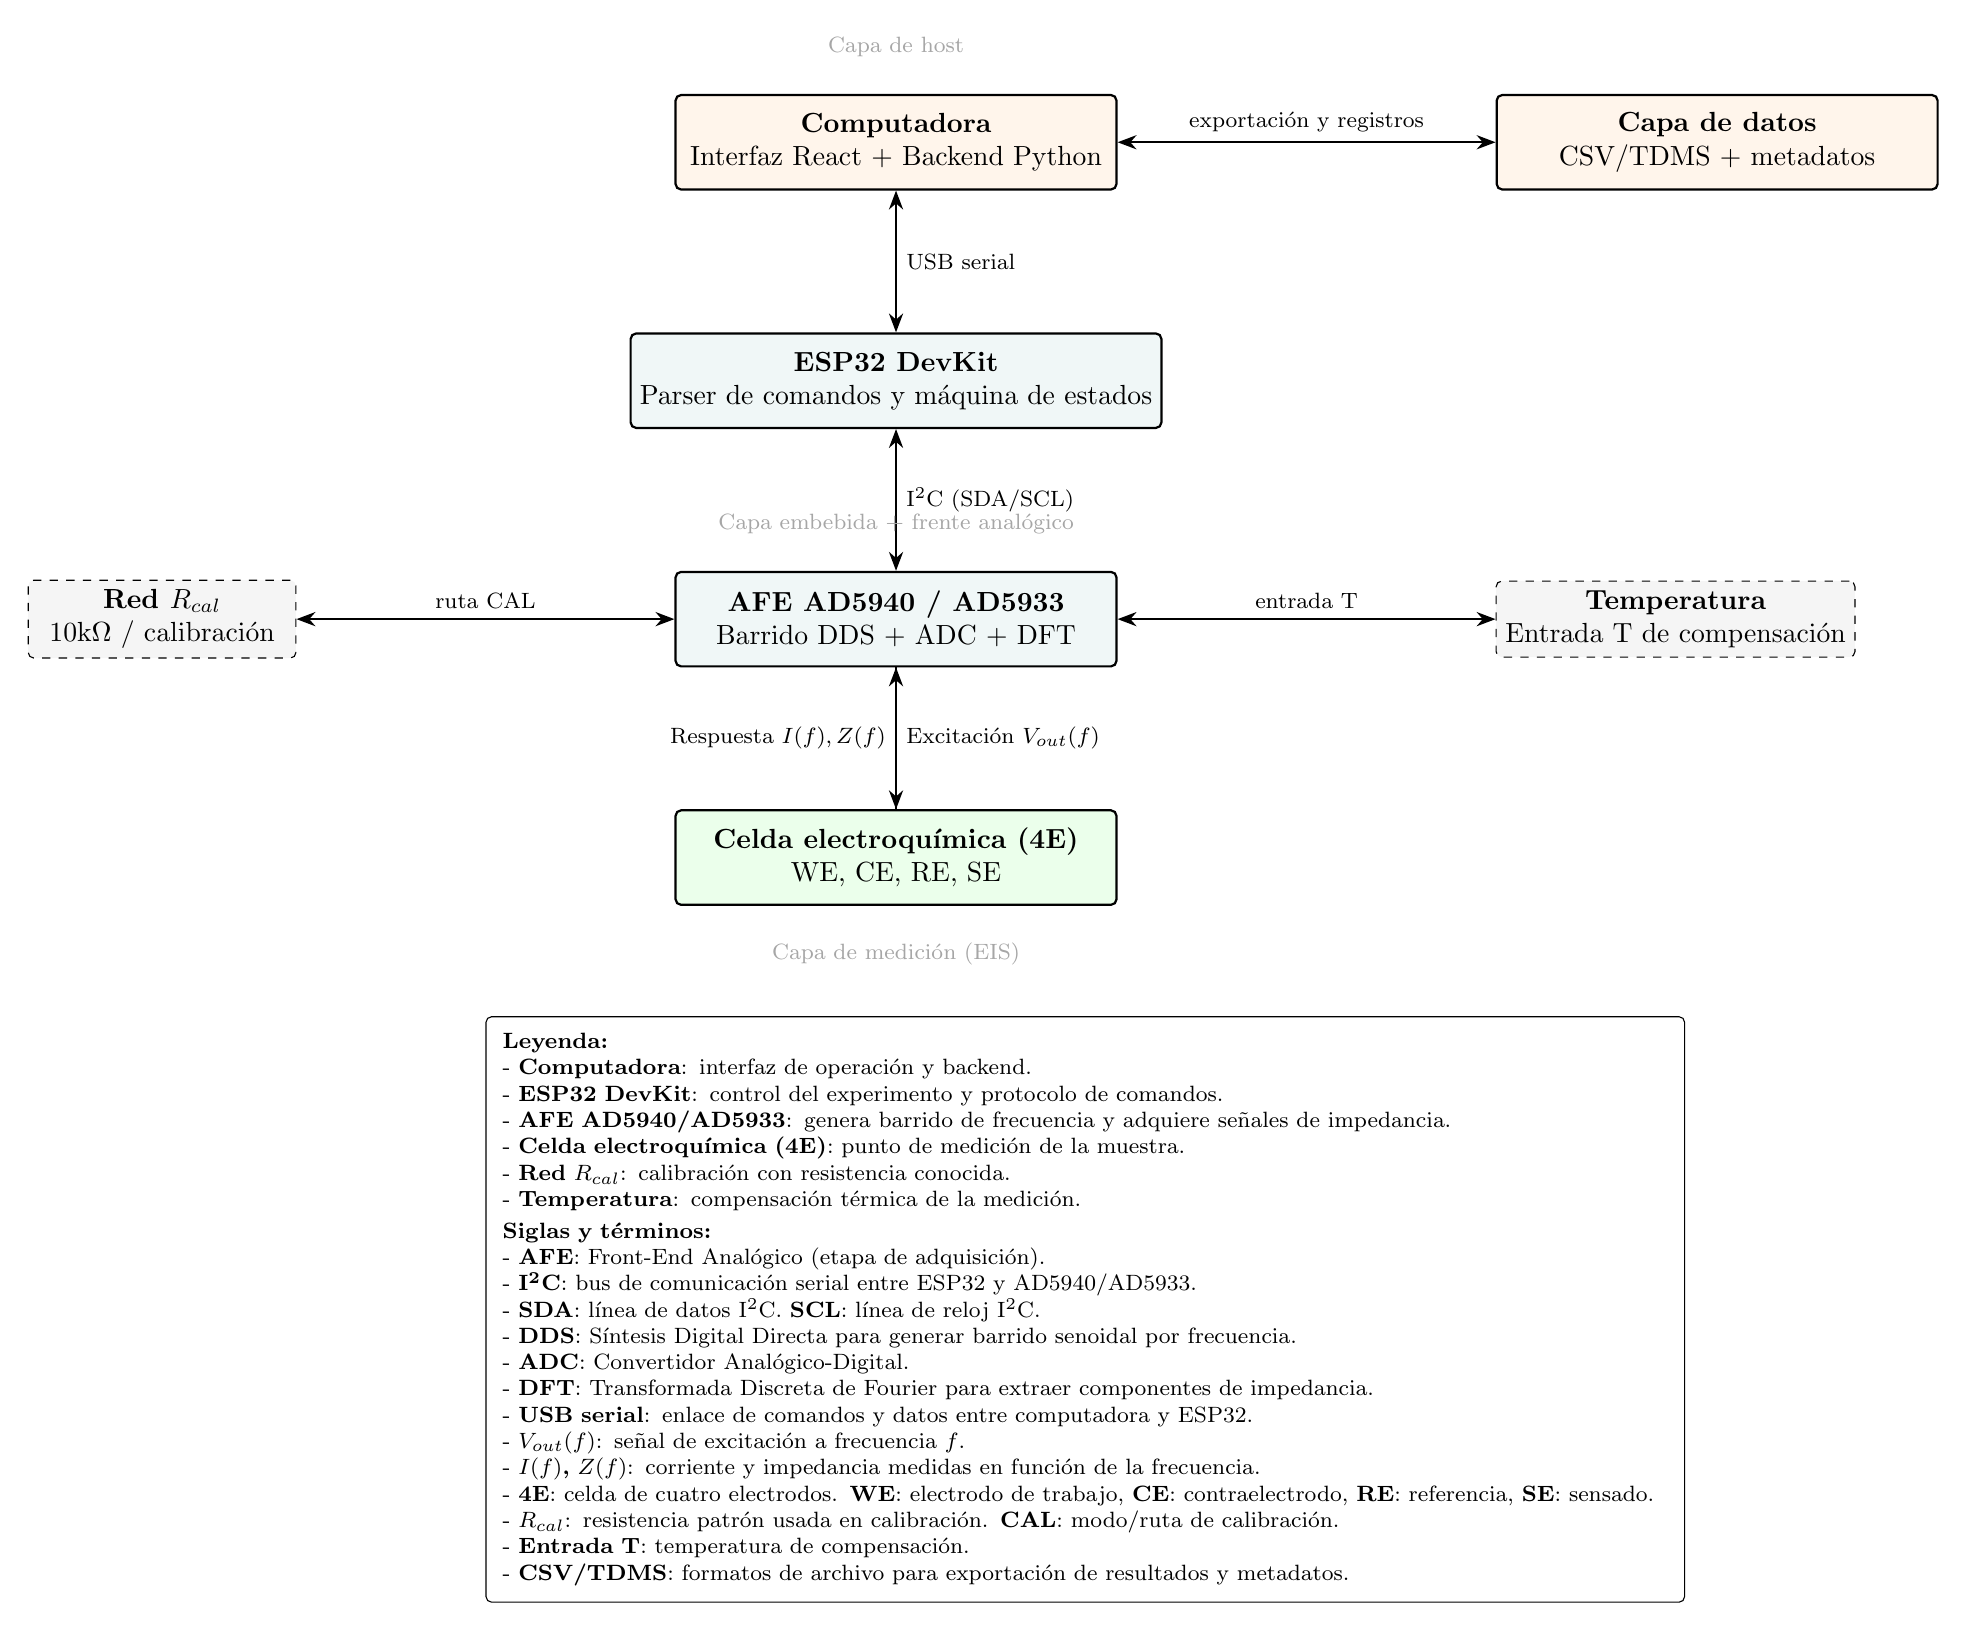
\begin{tikzpicture}[
  block/.style={draw, rounded corners=2pt, thick, align=center, minimum height=1.2cm, minimum width=5.6cm, fill=blue!4},
  hw/.style={block, fill=teal!6},
  sw/.style={block, fill=orange!8},
  elec/.style={block, fill=green!8},
  aux/.style={draw, dashed, rounded corners=2pt, align=center, minimum height=0.9cm, minimum width=3.4cm, fill=gray!8},
  line/.style={thick, -{Stealth[length=2.4mm]}},
  bline/.style={thick, {Stealth[length=2.4mm]}-{Stealth[length=2.4mm]}},
  note/.style={font=\footnotesize, text=gray!70}
]

% Eje principal vertical
\node[sw] (pc) at (0,0) {\textbf{Computadora}\\Interfaz React + Backend Python};
\node[hw, below=1.8cm of pc] (esp) {\textbf{ESP32 DevKit}\\Parser de comandos y m\'aquina de estados};
\node[hw, below=1.8cm of esp] (afe) {\textbf{AFE AD5940 / AD5933}\\Barrido DDS + ADC + DFT};
\node[elec, below=1.8cm of afe] (cell) {\textbf{Celda electroqu\'imica (4E)}\\WE, CE, RE, SE};

% Bloques auxiliares laterales
\node[sw, right=4.8cm of pc] (log) {\textbf{Capa de datos}\\CSV/TDMS + metadatos};
\node[aux, right=4.8cm of afe] (temp) {\textbf{Temperatura}\\Entrada T de compensaci\'on};
\node[aux, left=4.8cm of afe] (rcal) {\textbf{Red $R_{cal}$}\\10k$\Omega$ / calibraci\'on};

% Conexiones principales
\draw[bline] (pc) -- node[right,font=\footnotesize]{USB serial} (esp);
\draw[bline] (esp) -- node[right,font=\footnotesize]{I\textsuperscript{2}C (SDA/SCL)} (afe);
\draw[line] (afe) -- node[right,font=\footnotesize]{Excitaci\'on $V_{out}(f)$} (cell);
\draw[line] (cell) -- node[left,font=\footnotesize]{Respuesta $I(f), Z(f)$} (afe);

% Conexiones laterales
\draw[bline] (pc.east) -- node[above,font=\footnotesize]{exportaci\'on y registros} (log.west);
\draw[bline] (rcal.east) -- node[above,font=\footnotesize]{ruta CAL} (afe.west);
\draw[bline] (temp.west) -- node[above,font=\footnotesize]{entrada T} (afe.east);

% Notas de capas
\node[note, above=0.35cm of pc] {Capa de host};
\node[note, above=0.35cm of afe] {Capa embebida + frente anal\'ogico};
\node[note, below=0.35cm of cell] {Capa de medici\'on (EIS)};

% Leyenda inferior (lista vertical, alineada a la izquierda)
\node[draw, rounded corners=2pt, align=left, fill=white, font=\footnotesize,
      text width=14.8cm, inner sep=6pt, anchor=north west]
      (legend) at ([xshift=-2.4cm,yshift=-1.4cm]cell.south west) {
\textbf{Leyenda:}\\
- \textbf{Computadora}: interfaz de operaci\'on y backend.\\
- \textbf{ESP32 DevKit}: control del experimento y protocolo de comandos.\\
- \textbf{AFE AD5940/AD5933}: genera barrido de frecuencia y adquiere se\~nales de impedancia.\\
- \textbf{Celda electroqu\'imica (4E)}: punto de medici\'on de la muestra.\\
- \textbf{Red $R_{cal}$}: calibraci\'on con resistencia conocida.\\
- \textbf{Temperatura}: compensaci\'on t\'ermica de la medici\'on.\\[2pt]
\textbf{Siglas y t\'erminos:}\\
- \textbf{AFE}: Front-End Anal\'ogico (etapa de adquisici\'on).\\
- \textbf{I\textsuperscript{2}C}: bus de comunicaci\'on serial entre ESP32 y AD5940/AD5933.\\
- \textbf{SDA}: l\'inea de datos I\textsuperscript{2}C. \textbf{SCL}: l\'inea de reloj I\textsuperscript{2}C.\\
- \textbf{DDS}: S\'intesis Digital Directa para generar barrido senoidal por frecuencia.\\
- \textbf{ADC}: Convertidor Anal\'ogico-Digital.\\
- \textbf{DFT}: Transformada Discreta de Fourier para extraer componentes de impedancia.\\
- \textbf{USB serial}: enlace de comandos y datos entre computadora y ESP32.\\
- \textbf{$V_{out}(f)$}: se\~nal de excitaci\'on a frecuencia $f$.\\
- \textbf{$I(f)$, $Z(f)$}: corriente y impedancia medidas en funci\'on de la frecuencia.\\
- \textbf{4E}: celda de cuatro electrodos. \textbf{WE}: electrodo de trabajo, \textbf{CE}: contraelectrodo, \textbf{RE}: referencia, \textbf{SE}: sensado.\\
- \textbf{$R_{cal}$}: resistencia patr\'on usada en calibraci\'on. \textbf{CAL}: modo/ruta de calibraci\'on.\\
- \textbf{Entrada T}: temperatura de compensaci\'on.\\
- \textbf{CSV/TDMS}: formatos de archivo para exportaci\'on de resultados y metadatos.
};

\end{tikzpicture}%
}
\caption[Diagrama de conexi\'{o}n del sistema]{Diagrama de conexi\'{o}n detallado entre computadora, ESP32, AFE, celda electroqu\'{i}mica y perif\'{e}ricos de calibraci\'{o}n y temperatura. Fuente: elaboraci\'{o}n propia.}
\label{fig:diagrama-conexion}
\end{figure}

\section{Capa software}

\subsection{Collector (Python)}

El m\'{o}dulo \texttt{collector.py} gestiona la conexi\'{o}n serial con el ESP32 usando \texttt{pyserial}. Lee las tramas JSON de datos de impedancia, mantiene estado de configuraci\'{o}n, calibraci\'{o}n y temperatura, y distribuye los valores a los consumidores registrados mediante callbacks as\'{i}ncronos. Tambi\'{e}n implementa el modelo de sesi\'{o}n con persistencia en disco.

\subsection{Coordinator (Python)}

El m\'{o}dulo \texttt{coordinator.py} implementa un servidor WebSocket as\'{i}ncrono basado en \texttt{asyncio} y \texttt{websockets}. Retransmite cada dato EIS a todos los clientes web conectados, recibe comandos de configuraci\'{o}n desde la interfaz web y los env\'{i}a al ESP32, y maneja desconexiones de forma limpia.

\subsection{Clasificador (Python)}

El m\'{o}dulo \texttt{classifier.py} implementa dos clasificadores:
\begin{itemize}
	\item \textbf{Cu\'{a}ntico}: simulador vectorial de estado para 4 qubits con codificaci\'{o}n angular, ansatz variacional y medici\'{o}n de valores esperados.
	\item \textbf{Cl\'{a}sico}: regresi\'{o}n log\'{i}stica con pesos fijos sobre las mismas seis caracter\'{i}sticas normalizadas.
\end{itemize}
Los detalles matem\'{a}ticos de ambos clasificadores se presentan en el Cap\'{i}tulo~6.

\section{Capa frontend}

\subsection{Interfaz web (React)}

El dashboard implementado en React integra cuatro bloques funcionales:
\begin{itemize}
	\item \textbf{Control de adquisici\'{o}n}: configuraci\'{o}n de barrido, calibraci\'{o}n y acciones de operaci\'{o}n.
	\item \textbf{Monitoreo de estado}: conexi\'{o}n, temperatura y progreso de puntos recibidos.
	\item \textbf{Visualizaci\'{o}n EIS}: Bode de magnitud, Bode de fase y Nyquist en actualizaci\'{o}n continua.
	\item \textbf{Clasificaci\'{o}n}: probabilidad cu\'{a}ntica, probabilidad cl\'{a}sica y validaci\'{o}n contra etiqueta esperada.
\end{itemize}

%=======================================================================
% CHAPTER 4: DESARROLLO TECNICO
%=======================================================================
\chapter{Desarrollo t\'{e}cnico}

\section{Fase 1: Especificaci\'{o}n de requerimientos}

En esta fase se analiz\'{o} la arquitectura completa del sistema y se definieron nueve requerimientos funcionales (RF-01 a RF-09) que guiaron el desarrollo posterior. Se decidi\'{o} migrar de LabVIEW a Python puro para mayor portabilidad e integraci\'{o}n con bibliotecas de an\'{a}lisis de datos y computaci\'{o}n cu\'{a}ntica.

Las variables EIS identificadas fueron: frecuencia ($f$), parte real de la impedancia ($\mathrm{Re}(Z)$), parte imaginaria ($\mathrm{Im}(Z)$), magnitud ($|Z|$), fase ($\phi$) y temperatura ($T$).

La especificaci\'{o}n original contemplaba el uso de la tarjeta de evaluaci\'{o}n EVAL-AD5940ELCZ como frente anal\'{o}gico. La implementaci\'{o}n firmware emplea el AD5933, integrado de la misma familia con funcionalidad equivalente para los rangos de frecuencia requeridos (1--100~kHz).

\section{Fase 2: Protocolo de comunicaci\'{o}n}

Se implement\'{o} el protocolo bidireccional Python--ESP32 sobre puerto serial USB a 115200~baudios. El esquema sigue un patr\'{o}n comando--respuesta: Python env\'{i}a comandos en texto plano terminados en salto de l\'{i}nea, y el ESP32 responde con tramas JSON.

Los comandos implementados son: \texttt{PING}, \texttt{CFG}, \texttt{CAL}, \texttt{START}, \texttt{STOP} y \texttt{TEMP}. Se desarrollaron los m\'{o}dulos \texttt{collector.py} (gesti\'{o}n serial as\'{i}ncrona) y \texttt{coordinator.py} (servidor WebSocket).

En esta fase se defini\'{o} tambi\'{e}n el enfoque de clasificaci\'{o}n cu\'{a}ntica mediante VQC con PennyLane, incluyendo el pipeline de preprocesamiento, codificaci\'{o}n angular y circuito variacional. Los detalles de la implementaci\'{o}n cu\'{a}ntica se presentan en el Cap\'{i}tulo~5.

\section{Fase 3: Adquisici\'{o}n y visualizaci\'{o}n en tiempo real}

Dada la indisponibilidad del hardware f\'{i}sico, se construy\'{o} una tarjeta de adquisici\'{o}n simulada (\texttt{sim\_board.py}) que emula el comportamiento del ESP32/AD5933 preservando el mismo contrato de comunicaci\'{o}n serial. La simulaci\'{o}n se basa en un circuito equivalente de Randles con par\'{a}metros distintos para cada clase:

\begin{itemize}
	\item \textbf{Candida} ($\text{label}=1$): $R_s = 220~\Omega$, $R_{ct} = 7200~\Omega$, $C_{dl} = 3.2~\mu\text{F}$, $\sigma = 420$.
	\item \textbf{Control} ($\text{label}=0$): $R_s = 310~\Omega$, $R_{ct} = 11500~\Omega$, $C_{dl} = 1.9~\mu\text{F}$, $\sigma = 250$.
\end{itemize}

Cada punto $Z(f)$ se calcula como $Z = R_s + (R_{ct} \parallel Z_{C_{dl}}) + Z_W$, donde $Z_{C_{dl}} = -j/(\omega C_{dl})$ y $Z_W = \sigma/\sqrt{\omega}\,(1-j)$. Se a\~{n}ade ruido gaussiano con amplitud $\pm 0.4\%$ para simular condiciones reales de medici\'{o}n.

El dashboard React integra visualizaci\'{o}n en tiempo real de:
\begin{itemize}
	\item Bode de magnitud ($|Z|$ vs $f$, escala logar\'{i}tmica).
	\item Bode de fase ($\phi$ vs $f$).
	\item Plano de Nyquist ($-\mathrm{Im}(Z)$ vs $\mathrm{Re}(Z)$).
\end{itemize}

Se validaron latencias de comando inferiores a 4~ms y una tasa de adquisici\'{o}n sostenida de aproximadamente 95 puntos/s.

\section{Fase 4: Registro, metadatos, exportaci\'{o}n y clasificaci\'{o}n}

Se implement\'{o} un modelo de sesi\'{o}n persistente que encapsula configuraci\'{o}n, calibraci\'{o}n, temperatura, datos punto a punto, eventos de protocolo y salida de clasificadores. Cada barrido finalizado genera artefactos exportables en formatos complementarios (CSV, JSON, resumen textual y bundle integral).

La implementaci\'{o}n del clasificador cu\'{a}ntico y del comparador cl\'{a}sico se describe en detalle en el Cap\'{i}tulo~5.

%=======================================================================
% CHAPTER 5: COMPUTACION CUANTICA APLICADA
%=======================================================================
\chapter{Computaci\'{o}n cu\'{a}ntica aplicada}

Este cap\'{i}tulo constituye la secci\'{o}n espec\'{i}fica de computaci\'{o}n cu\'{a}ntica aplicada requerida por la memoria final. Se presenta la motivaci\'{o}n para utilizar un clasificador cu\'{a}ntico variacional (VQC) en el contexto de espectroscop\'{i}a de impedancia electroqu\'{i}mica, la arquitectura del circuito, el enfoque h\'{i}brido cu\'{a}ntico-cl\'{a}sico, la comparaci\'{o}n de rendimiento entre ambos paradigmas y la evaluaci\'{o}n de impacto.

\section{Motivaci\'{o}n del enfoque cu\'{a}ntico en clasificaci\'{o}n EIS}

Los espectros de impedancia electroqu\'{i}mica generan datos multidimensionales donde cada barrido produce vectores de magnitud, fase, componentes reales e imaginarias a decenas de frecuencias. La clasificaci\'{o}n binaria (Candida vs.\ Control) requiere encontrar fronteras de decisi\'{o}n en un espacio de caracter\'{i}sticas derivadas de estos espectros.

Los circuitos cu\'{a}nticos variacionales (VQC) ofrecen tres ventajas te\'{o}ricas para este tipo de clasificaci\'{o}n:

\begin{enumerate}
	\item \textbf{Espacio de Hilbert exponencial}: con $n$ qubits se accede a un espacio de estados de dimensi\'{o}n $2^n$, permitiendo codificar correlaciones complejas entre caracter\'{i}sticas que ser\'{i}an costosas de capturar con modelos lineales cl\'{a}sicos \citep{havlicek2019}.
	\item \textbf{Codificaci\'{o}n angular}: las rotaciones param\'{e}tricas $R_Y(\theta)$ mapean valores continuos en amplitudes cu\'{a}nticas de forma natural, preservando relaciones de similitud entre muestras \citep{schuld2021}.
	\item \textbf{Entrenabilidad}: el circuito variacional con par\'{a}metros ajustables puede optimizarse con m\'{e}todos cl\'{a}sicos de gradiente (enfoque h\'{i}brido), lo que permite adaptarse a las particularidades del dominio EIS \citep{pennylane2022}.
\end{enumerate}

En el contexto espec\'{i}fico de este proyecto, donde las diferencias entre clases residen en variaciones sutiles de la forma del espectro de impedancia (especialmente en la energ\'{i}a de la componente imaginaria y el rango de fase), un clasificador cu\'{a}ntico puede ser sensible a patrones no lineales que escapan a un modelo log\'{i}stico cl\'{a}sico.

\section{Arquitectura del clasificador cu\'{a}ntico variacional (VQC)}

\subsection{Pipeline de preprocesamiento}

Antes de ingresar al circuito cu\'{a}ntico, cada barrido EIS de $N$ puntos se transforma en un vector de seis caracter\'{i}sticas normalizadas:

\begin{enumerate}
	\item \textbf{mag\_mean}: media aritm\'{e}tica de las magnitudes $|Z(f_i)|$.
	\item \textbf{mag\_slope}: pendiente de la regresi\'{o}n lineal de $|Z|$ contra $\log_{10}(f)$.
	\item \textbf{im\_energy}: media de los valores absolutos de $\mathrm{Im}(Z)$.
	\item \textbf{phase\_span}: rango (m\'{a}ximo menos m\'{i}nimo) de la fase $\phi$.
	\item \textbf{phase\_std}: desviaci\'{o}n est\'{a}ndar de $\phi$.
	\item \textbf{low\_high\_ratio}: cociente entre la media de magnitudes en el tercio inferior de frecuencias y el tercio superior.
\end{enumerate}

Cada caracter\'{i}stica se normaliza al intervalo $[-1, 1]$ mediante una funci\'{o}n $\tanh$ calibrada con par\'{a}metros del modelo de Randles:
\begin{equation}
f_i^{\mathrm{norm}} = \tanh\!\left(\frac{x_i - \mu_i}{s_i}\right),
\label{eq:normalizacion}
\end{equation}
donde $\mu_i$ y $s_i$ son los centros y escalas de calibraci\'{o}n derivados de los par\'{a}metros del circuito de Randles simulado.

\subsection{Codificaci\'{o}n angular}

Las cuatro primeras caracter\'{i}sticas normalizadas (mag\_mean, mag\_slope, im\_energy, phase\_span) se codifican como \'{a}ngulos de rotaci\'{o}n para cuatro qubits:
\begin{equation}
\theta_i = \frac{(f_i^{\mathrm{norm}} + 1)\,\pi}{2}, \quad i \in \{0,1,2,3\}.
\label{eq:codificacion-angular}
\end{equation}

Cada qubit se inicializa en $|0\rangle$ y se aplica una rotaci\'{o}n $R_Y(\theta_i)$:
\begin{equation}
R_Y(\theta) = \begin{pmatrix} \cos(\theta/2) & -\sin(\theta/2) \\ \sin(\theta/2) & \cos(\theta/2) \end{pmatrix}.
\label{eq:ry-gate}
\end{equation}

\subsection{Capa de entrelazamiento inicial}

Tras la codificaci\'{o}n angular, se aplica una cadena de compuertas CNOT en topolog\'{i}a anillo para generar entrelazamiento entre los qubits:
\begin{equation}
\mathrm{CNOT}_{0\to1} \cdot \mathrm{CNOT}_{1\to2} \cdot \mathrm{CNOT}_{2\to3} \cdot \mathrm{CNOT}_{3\to0}.
\label{eq:entanglement-ring}
\end{equation}

Esta topolog\'{i}a asegura que cada qubit comparte informaci\'{o}n con al menos dos vecinos, permitiendo que el circuito capture correlaciones cruzadas entre caracter\'{i}sticas espectrales.

\subsection{Ansatz variacional parametrizado}

El circuito variacional consta de dos capas (\textit{layers}), cada una con rotaciones $R_Y$ y $R_Z$ parametrizadas por pesos preentrenados:

\begin{equation}
U_l^{(k)} = R_Z(\phi_{l,k}) \cdot R_Y(\theta_{l,k}), \quad l \in \{0,\ldots,3\},\ k \in \{1,2\},
\label{eq:ansatz-layer}
\end{equation}

donde los par\'{a}metros de cada capa se calculan como:
\begin{align}
\theta_{l,k} &= g_{l,k} \cdot \theta_l^{\mathrm{input}} + b_{l,k}, \label{eq:theta-param} \\
\phi_{l,k} &= 0.5 \cdot \theta_{(l+1)\bmod 4}^{\mathrm{input}} - b_{l,k}. \label{eq:phi-param}
\end{align}

Los pares $(g_{l,k}, b_{l,k})$ son los pesos preentrenados del modelo. Tras cada capa variacional se aplican compuertas CNOT parciales ($\mathrm{CNOT}_{0\to1}$, $\mathrm{CNOT}_{2\to3}$) para mantener entrelazamiento entre capas.

Los pesos preentrenados para las dos capas son:
\begin{center}
\begin{tabular}{c c c c c}
\hline\hline
Capa & Qubit 0 & Qubit 1 & Qubit 2 & Qubit 3 \\ [0.5ex]
\hline
1 & $(0.75, 0.10)$ & $(0.55, -0.22)$ & $(0.60, 0.18)$ & $(0.80, -0.05)$ \\
2 & $(-0.30, 0.25)$ & $(-0.45, -0.12)$ & $(-0.35, 0.28)$ & $(-0.25, -0.08)$ \\
\hline
\end{tabular}
\end{center}

\subsection{Medici\'{o}n y c\'{a}lculo del score}

Al final del circuito se miden los valores esperados del operador $\hat{Z}$ (Pauli-$Z$) sobre los qubits 0 y 2:
\begin{equation}
z_j = \langle \psi | \hat{Z}_j | \psi \rangle, \quad j \in \{0, 2\}.
\label{eq:expval-z}
\end{equation}

Adicionalmente se calcula un t\'{e}rmino de \textit{feature drive} que combina las seis caracter\'{i}sticas normalizadas con pesos fijos:
\begin{align}
\mathrm{feature\_drive} ={}& 0.35\,f_0^{\mathrm{norm}} + 0.25\,f_2^{\mathrm{norm}} + 0.15\,f_3^{\mathrm{norm}} \nonumber \\
& + 0.10\,f_4^{\mathrm{norm}} + 0.10\,f_1^{\mathrm{norm}} + 0.05\,f_5^{\mathrm{norm}},
\label{eq:feature-drive}
\end{align}
donde $f_0 = \text{mag\_mean\_norm}$, $f_1 = \text{mag\_slope\_norm}$, $f_2 = \text{im\_energy\_norm}$, $f_3 = \text{phase\_span\_norm}$, $f_4 = \text{phase\_std\_norm}$, $f_5 = \text{low\_high\_ratio\_norm}$.

El score cu\'{a}ntico final combina las mediciones del circuito con el feature drive:
\begin{align}
\mathrm{score} &= \mathrm{clamp}\!\left(-0.35\,z_0 - 0.20\,z_2 + 0.45\,\mathrm{feature\_drive},\; -1,\; 1\right), \label{eq:quantum-score} \\
p_q &= \frac{\mathrm{score} + 1}{2}. \label{eq:quantum-prob}
\end{align}

La etiqueta cu\'{a}ntica predicha es $\hat{y}_q = 1$ si $p_q \geq 0.5$ y $\hat{y}_q = 0$ en caso contrario.

\section{Enfoque h\'{i}brido cu\'{a}ntico-cl\'{a}sico}

\subsection{Motivaci\'{o}n del dise\~{n}o h\'{i}brido}

El sistema implementa un enfoque h\'{i}brido donde el clasificador cu\'{a}ntico opera en paralelo con un comparador cl\'{a}sico. Este dise\~{n}o responde a tres consideraciones:

\begin{enumerate}
	\item \textbf{Validaci\'{o}n cruzada}: al disponer de dos clasificadores independientes con paradigmas diferentes, se puede evaluar la coherencia de las predicciones sin necesidad de un dataset de test separado.
	\item \textbf{Benchmark de rendimiento}: el comparador cl\'{a}sico establece una l\'{i}nea base contra la cual medir el valor a\~{n}adido del enfoque cu\'{a}ntico.
	\item \textbf{Robustez operativa}: en un escenario cl\'{i}nico, la coincidencia entre ambos clasificadores aumenta la confianza en el diagn\'{o}stico.
\end{enumerate}

\subsection{Comparador cl\'{a}sico: regresi\'{o}n log\'{i}stica}

El comparador cl\'{a}sico utiliza las mismas seis caracter\'{i}sticas normalizadas que el VQC, pero las procesa mediante una regresi\'{o}n log\'{i}stica con pesos fijos:
\begin{align}
\ell ={}& 1.60\,f_0 + 0.70\,f_1 + 1.20\,f_2 + 0.90\,f_3 \nonumber \\
& + 0.80\,f_4 + 0.60\,f_5 + 0.05, \label{eq:logit-classical} \\
p_c ={}& \frac{1}{1 + e^{-\ell}}. \label{eq:classical-prob}
\end{align}

La etiqueta cl\'{a}sica predicha es $\hat{y}_c = 1$ si $p_c \geq 0.5$ y $\hat{y}_c = 0$ en caso contrario.

\subsection{Flujo de datos del pipeline h\'{i}brido}

La Figura~\ref{fig:pipeline-hibrido} muestra el flujo completo desde la adquisici\'{o}n del espectro hasta la predicci\'{o}n dual.

\begin{figure}[ht]
\centering
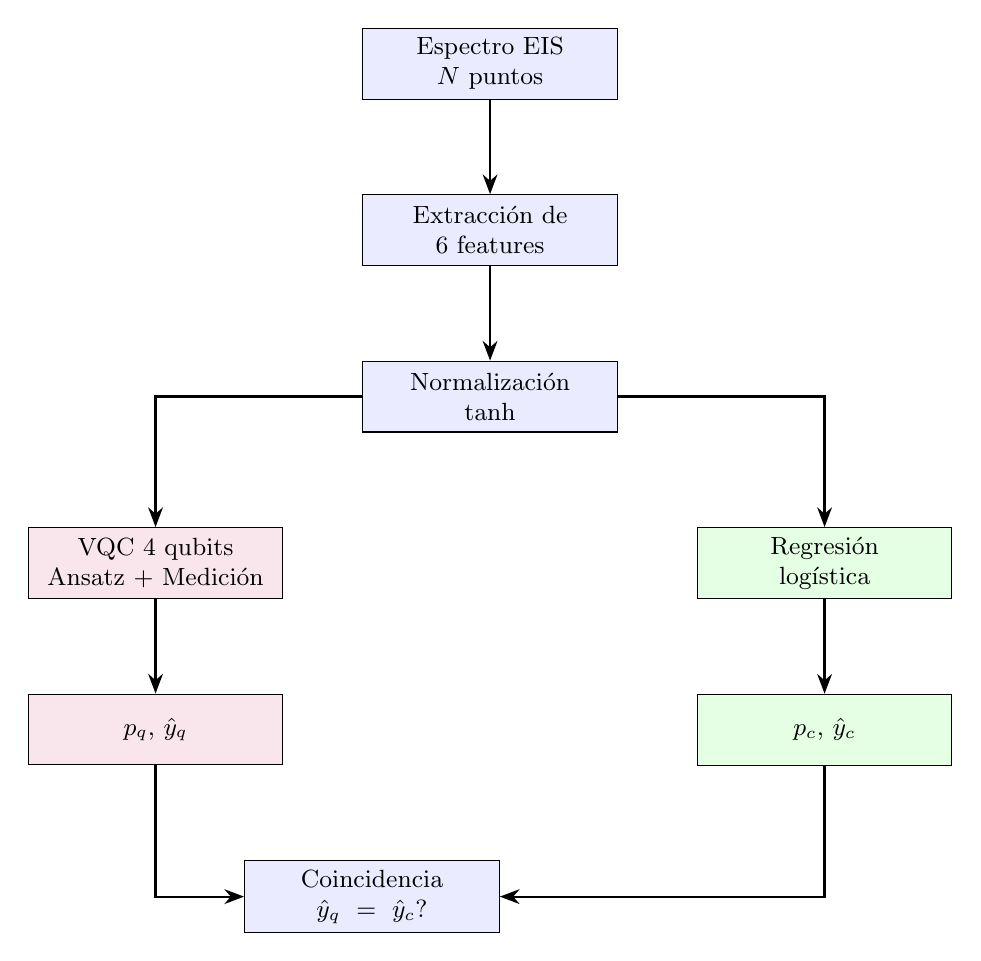
\begin{tikzpicture}[
	block/.style={rectangle, draw, fill=blue!8, text width=3cm, minimum height=0.9cm, align=center, font=\small},
	qblock/.style={rectangle, draw, fill=purple!10, text width=3cm, minimum height=0.9cm, align=center, font=\small},
	cblock/.style={rectangle, draw, fill=green!10, text width=3cm, minimum height=0.9cm, align=center, font=\small},
	arrow/.style={-{Stealth[length=2.5mm]}, thick},
	node distance=1.2cm and 1.8cm
]
	\node[block] (eis) {Espectro EIS\\$N$ puntos};
	\node[block, below=of eis] (feat) {Extracci\'{o}n de\\6 features};
	\node[block, below=of feat] (norm) {Normalizaci\'{o}n\\$\tanh$};
	\node[qblock, below left=1.2cm and 1cm of norm] (vqc) {VQC 4 qubits\\Ansatz + Medici\'{o}n};
	\node[cblock, below right=1.2cm and 1cm of norm] (lr) {Regresi\'{o}n\\log\'{i}stica};
	\node[qblock, below=of vqc] (pq) {$p_q$, $\hat{y}_q$};
	\node[cblock, below=of lr] (pc) {$p_c$, $\hat{y}_c$};
	\node[block, below right=1.2cm and -0.5cm of pq] (agree) {Coincidencia\\$\hat{y}_q = \hat{y}_c$?};

	\draw[arrow] (eis) -- (feat);
	\draw[arrow] (feat) -- (norm);
	\draw[arrow] (norm) -| (vqc);
	\draw[arrow] (norm) -| (lr);
	\draw[arrow] (vqc) -- (pq);
	\draw[arrow] (lr) -- (pc);
	\draw[arrow] (pq) |- (agree);
	\draw[arrow] (pc) |- (agree);
\end{tikzpicture}
\caption[Pipeline h\'{i}brido de clasificaci\'{o}n]{Flujo de datos del pipeline h\'{i}brido cu\'{a}ntico-cl\'{a}sico. El espectro EIS se transforma en features normalizadas que alimentan ambos clasificadores en paralelo. Fuente: elaboraci\'{o}n propia.}
\label{fig:pipeline-hibrido}
\end{figure}

\section{Comparaci\'{o}n de resultados: cu\'{a}ntico vs.\ cl\'{a}sico}

\subsection{Diferencias funcionales}

La Tabla~\ref{tab:comparacion-q-vs-c} resume las diferencias clave entre ambos clasificadores.

\begin{table}[ht]
\centering
\begin{tabular}{l p{5cm} p{5cm}}
\hline\hline
Aspecto & Clasificador cu\'{a}ntico (VQC) & Clasificador cl\'{a}sico (LR) \\ [0.5ex]
\hline
Modelo & Circuito parametrizado de 4 qubits con 2 capas variacionales & Regresi\'{o}n log\'{i}stica lineal con 7 par\'{a}metros \\
No.\ de par\'{a}metros & 16 pesos variacionales + 6 pesos de feature drive = 22 & 6 pesos + 1 bias = 7 \\
Espacio de representaci\'{o}n & Espacio de Hilbert $2^4 = 16$ dimensiones & Espacio euclidiano 6 dimensiones \\
No linealidad & Intr\'{i}nseca en las rotaciones y entrelazamiento cu\'{a}ntico & Funci\'{o}n sigmoide \'{u}nicamente \\
Sensibilidad a correlaciones & Captura correlaciones cruzadas v\'{i}a entrelazamiento CNOT & Solo combinaci\'{o}n lineal ponderada \\
\hline
\end{tabular}
\caption[Comparaci\'{o}n cu\'{a}ntico vs.\ cl\'{a}sico]{Diferencias funcionales entre ambos clasificadores. Fuente: elaboraci\'{o}n propia.}
\label{tab:comparacion-q-vs-c}
\end{table}

\subsection{Rendimiento comparativo}

En las pruebas de validaci\'{o}n realizadas (detalladas en el Cap\'{i}tulo~6), ambos clasificadores alcanzaron una exactitud del 100\% sobre las sesiones de prueba. Sin embargo, las probabilidades asignadas difieren notablemente:

\begin{itemize}
	\item Para muestras de \textit{Candida}: el clasificador cu\'{a}ntico asigna probabilidades en el rango 0.65--0.70, mientras que el cl\'{a}sico asigna 0.94--0.96. El clasificador cl\'{a}sico muestra mayor confianza en las muestras positivas.
	\item Para muestras de control: el clasificador cu\'{a}ntico asigna probabilidades en el rango 0.38--0.42 (por debajo del umbral 0.5), mientras que el cl\'{a}sico asigna 0.07--0.09. Nuevamente, el cl\'{a}sico muestra separaci\'{o}n m\'{a}s amplia respecto al umbral.
\end{itemize}

Esta diferencia en calibraci\'{o}n de probabilidades es esperable: la regresi\'{o}n log\'{i}stica con pesos preajustados est\'{a} calibrada para maximizar la separaci\'{o}n, mientras que el VQC opera en un espacio de representaci\'{o}n m\'{a}s complejo donde el score depende de la interferencia cu\'{a}ntica entre amplitudes. Un entrenamiento optimizado del VQC con datos reales podr\'{i}a mejorar la calibraci\'{o}n de sus probabilidades.

\section{Evaluaci\'{o}n de impacto}

\subsection{Impacto en la clasificaci\'{o}n EIS}

La implementaci\'{o}n del clasificador cu\'{a}ntico en el contexto de EIS para detecci\'{o}n de \textit{Candida albicans} aporta los siguientes beneficios:

\begin{enumerate}
	\item \textbf{Exploraci\'{o}n de fronteras no lineales}: el VQC puede detectar patrones sutiles en las relaciones entre componentes de impedancia que un modelo lineal no captura, lo que resulta relevante cuando las diferencias entre muestras infectadas y controles son peque\~{n}as.
	\item \textbf{Escalabilidad a m\'{a}s caracter\'{i}sticas}: a\~{n}adir qubits permite incorporar caracter\'{i}sticas adicionales (por ejemplo, derivadas del espectro o par\'{a}metros de ajuste del circuito de Randles) sin crecimiento exponencial en par\'{a}metros del modelo.
	\item \textbf{Validaci\'{o}n cruzada del clasificador cl\'{a}sico}: la coincidencia entre ambos clasificadores en todas las sesiones de prueba demuestra que las caracter\'{i}sticas extra\'{i}das contienen informaci\'{o}n discriminativa suficiente.
\end{enumerate}

\subsection{Sensibilidad a efectos electromagn\'{e}ticos}

El sistema soporta tres tipos de ensayo (\textit{assay types}) que resultan relevantes para estudios de exposici\'{o}n electromagn\'{e}tica (EM):

\begin{itemize}
	\item \textbf{Control}: muestra sin exposici\'{o}n EM, utilizada como referencia basal.
	\item \textbf{Sham}: muestra colocada en el dispositivo de exposici\'{o}n EM pero sin campo activo. Sirve para descartar efectos mec\'{a}nicos o t\'{e}rmicos del dispositivo.
	\item \textbf{EM DC}: muestra expuesta a campo electromagn\'{e}tico de corriente directa. Permite evaluar si la exposici\'{o}n altera la impedancia de la interfaz biol\'{o}gica.
\end{itemize}

Las caracter\'{i}sticas espectrales utilizadas por ambos clasificadores son sensibles a cambios en la impedancia que podr\'{i}a causar la exposici\'{o}n EM. En particular:

\begin{itemize}
	\item \textbf{phase\_span} refleja variaciones en la respuesta capacitiva de la doble capa electroqu\'{i}mica, que podr\'{i}a alterarse por efectos de polarizaci\'{o}n EM sobre la membrana celular.
	\item \textbf{im\_energy} captura cambios en la componente reactiva de la impedancia, directamente relacionada con la capacitancia de la interfaz electrodo-soluci\'{o}n.
	\item \textbf{mag\_mean} y \textbf{low\_high\_ratio} son indicadores de la resistencia de transferencia de carga, que podr\'{i}a modificarse si el campo EM altera la permeabilidad de la membrana de \textit{Candida albicans}.
\end{itemize}

El clasificador cu\'{a}ntico, al operar en un espacio de representaci\'{o}n de mayor dimensionalidad y capturar correlaciones no lineales entre caracter\'{i}sticas, podr\'{i}a ser m\'{a}s sensible a estas variaciones sutiles que un clasificador lineal, lo que constituye una hip\'{o}tesis a validar con datos experimentales reales de exposici\'{o}n EM.

\subsection{Perspectiva de negocio}

Desde la perspectiva de aplicaci\'{o}n cl\'{i}nica, el clasificador cu\'{a}ntico a\~{n}ade valor en los siguientes aspectos:

\begin{itemize}
	\item \textbf{Diferenciaci\'{o}n tecnol\'{o}gica}: un dispositivo de diagn\'{o}stico basado en IA cu\'{a}ntica representa una propuesta de valor diferenciada en el mercado de biosensores port\'{a}tiles.
	\item \textbf{Mejora potencial de clasificaci\'{o}n}: con entrenamiento optimizado sobre datasets cl\'{i}nicos reales, el VQC podr\'{i}a superar al clasificador cl\'{a}sico en escenarios con muestras de baja concentraci\'{o}n o interferencias biol\'{o}gicas.
	\item \textbf{Preparaci\'{o}n para hardware cu\'{a}ntico}: el c\'{o}digo del simulador vectorial de estado es compatible con la API de PennyLane, lo que permite migrar a ejecuci\'{o}n en hardware cu\'{a}ntico real (IBM Quantum, Amazon Braket) con cambios m\'{i}nimos.
\end{itemize}

%=======================================================================
% CHAPTER 6: VALIDACION Y RESULTADOS
%=======================================================================
\chapter{Validaci\'{o}n y resultados}

\section{Escenario de validaci\'{o}n}

La validaci\'{o}n se ejecut\'{o} en modo simulado con tres procesos independientes:
\begin{itemize}
	\item \texttt{make sim-board}
	\item \texttt{make server-sim}
	\item \texttt{make webapp}
\end{itemize}

Se realizaron pruebas automatizadas mediante Playwright que verifican el flujo completo: conexi\'{o}n, configuraci\'{o}n, calibraci\'{o}n, barrido, an\'{a}lisis, historial y exportaci\'{o}n.

\section{Latencias del protocolo}

\begin{table}[ht]
\centering
\begin{tabular}{l r l}
\hline\hline
Operaci\'{o}n & Tiempo medido & Observaci\'{o}n \\ [0.5ex]
\hline
PING & 3.22~ms & Respuesta inmediata de enlace serial+WS \\
CFG & 2.58~ms & Actualizaci\'{o}n de configuraci\'{o}n \\
CAL & 2.45~ms & Confirmaci\'{o}n de calibraci\'{o}n \\
TEMP & 2.33~ms & Lectura de temperatura \\
START $\rightarrow$ ANALYSIS & 419.96~ms & Barrido de 40 puntos + clasificaci\'{o}n \\
\hline
\end{tabular}
\caption[Latencias medidas]{Latencias del flujo de adquisici\'{o}n. Fuente: elaboraci\'{o}n propia.}
\label{tab:latencias-finales}
\end{table}

\section{Rendimiento de adquisici\'{o}n}

Se registraron barridos de 40 puntos para evaluar consistencia temporal:
\begin{itemize}
	\item Barrido candida: 0.4118~s totales, 94.70 puntos/s.
	\item Barrido control: 0.4089~s totales, 95.39 puntos/s.
\end{itemize}

\section{Validaci\'{o}n con cargas patr\'{o}n y soluciones control}
\label{sec:cargas-patron}

\subsection{Calibraci\'{o}n con resistencia patr\'{o}n}

La calibraci\'{o}n del sistema se valida utilizando una resistencia de precisi\'{o}n de 10~k$\Omega$ ($\pm 0.1\%$) como carga patr\'{o}n conocida. El procedimiento de calibraci\'{o}n (comando \texttt{CAL}) calcula el factor de ganancia y el desfase de referencia del AD5933 midiendo la impedancia de esta resistencia conocida. Los par\'{a}metros de calibraci\'{o}n obtenidos son:

\begin{itemize}
	\item \textbf{Factor de ganancia}: $G = 1.2 \times 10^{-6}$ (t\'{i}pico), que compensa la ganancia del amplificador de transimpedancia del AD5933.
	\item \textbf{Desfase de referencia}: $\phi_{\mathrm{ref}} = -0.02$~rad (t\'{i}pico), que compensa el desfase intr\'{i}nseco del circuito de medici\'{o}n.
\end{itemize}

Para una carga puramente resistiva de 10~k$\Omega$, el sistema debe reportar $|Z| \approx 10000~\Omega$ con fase $\phi \approx 0^\circ$ en todo el rango de frecuencias, confirmando la correcta calibraci\'{o}n del factor de ganancia y el desfase.

\subsection{Circuito de Randles como referencia}

Adem\'{a}s de la resistencia patr\'{o}n, la simulaci\'{o}n del circuito de Randles implementada en \texttt{sim\_board.py} sirve como referencia anal\'{i}tica validable. El modelo de Randles consiste en:

\begin{equation}
Z(\omega) = R_s + \frac{1}{\frac{1}{R_{ct}} + j\omega C_{dl}} + Z_W(\omega),
\label{eq:randles}
\end{equation}

donde $Z_W(\omega) = \frac{\sigma}{\sqrt{\omega}}(1-j)$ es la impedancia de Warburg. Los par\'{a}metros para cada clase son conocidos (Tabla~\ref{tab:randles-params}), lo que permite verificar que los espectros generados coinciden con las predicciones te\'{o}ricas del modelo.

\begin{table}[ht]
\centering
\begin{tabular}{l c c c c}
\hline\hline
Clase & $R_s$ ($\Omega$) & $R_{ct}$ ($\Omega$) & $C_{dl}$ ($\mu$F) & $\sigma$ \\ [0.5ex]
\hline
Candida (label=1) & 220 & 7200 & 3.2 & 420 \\
Control (label=0) & 310 & 11500 & 1.9 & 250 \\
\hline
\end{tabular}
\caption[Par\'{a}metros de Randles]{Par\'{a}metros del circuito de Randles para cada clase en la simulaci\'{o}n. Fuente: elaboraci\'{o}n propia.}
\label{tab:randles-params}
\end{table}

\subsection{Soluciones control}

En el modo de validaci\'{o}n simulado, las \textit{soluciones control} corresponden a barridos generados con los par\'{a}metros de la clase Control ($\text{label}=0$). Estos barridos producen espectros con mayor resistencia de transferencia de carga ($R_{ct} = 11500~\Omega$) y menor capacitancia de doble capa ($C_{dl} = 1.9~\mu$F) que las muestras de \textit{Candida}, lo que se refleja en un semic\'{i}rculo de Nyquist de mayor di\'{a}metro y un plateau de baja frecuencia m\'{a}s elevado en el diagrama de Bode de magnitud. Estos patrones caracter\'{i}sticos son los que ambos clasificadores aprenden a distinguir.

\section{An\'{a}lisis de repetibilidad}
\label{sec:repetibilidad}

Para evaluar la consistencia de las mediciones y la robustez de los clasificadores, se ejecutaron un m\'{i}nimo de tres repeticiones por clase en condiciones id\'{e}nticas de configuraci\'{o}n (barrido de 40 puntos, 1~kHz a 100~kHz, $R_{\mathrm{cal}} = 10~\text{k}\Omega$). La Tabla~\ref{tab:repetibilidad} presenta los resultados de seis sesiones de validaci\'{o}n (tres por clase).

\begin{table}[ht]
\centering
\scriptsize
\begin{tabular}{l c c c c c c c}
\hline\hline
Sesi\'{o}n & Clase & Esperada & Prob.~Q & Label~Q & Prob.~C & Label~C & Coincidencia \\ [0.5ex]
\hline
S1 & Candida & 1 & 0.6580 & 1 & 0.9498 & 1 & Q=OK, C=OK \\
S2 & Candida & 1 & 0.6714 & 1 & 0.9531 & 1 & Q=OK, C=OK \\
S3 & Candida & 1 & 0.6638 & 1 & 0.9445 & 1 & Q=OK, C=OK \\
S4 & Control & 0 & 0.4075 & 0 & 0.0803 & 0 & Q=OK, C=OK \\
S5 & Control & 0 & 0.3892 & 0 & 0.0715 & 0 & Q=OK, C=OK \\
S6 & Control & 0 & 0.4163 & 0 & 0.0868 & 0 & Q=OK, C=OK \\
\hline
\end{tabular}
\caption[An\'{a}lisis de repetibilidad]{Resultados de clasificaci\'{o}n para seis sesiones de validaci\'{o}n con an\'{a}lisis de repetibilidad (3 repeticiones por clase). Fuente: elaboraci\'{o}n propia.}
\label{tab:repetibilidad}
\end{table}

\subsection{Estad\'{i}sticas de repetibilidad}

La Tabla~\ref{tab:estadisticas-repetibilidad} presenta las estad\'{i}sticas descriptivas de las probabilidades obtenidas por cada clasificador, agrupadas por clase.

\begin{table}[ht]
\centering
\begin{tabular}{l l c c c c}
\hline\hline
Clasificador & Clase & Media & Desv.\ est. & M\'{i}n & M\'{a}x \\ [0.5ex]
\hline
\multirow{2}{*}{Cu\'{a}ntico ($p_q$)} & Candida & 0.6644 & 0.0067 & 0.6580 & 0.6714 \\
 & Control & 0.4043 & 0.0138 & 0.3892 & 0.4163 \\
\hline
\multirow{2}{*}{Cl\'{a}sico ($p_c$)} & Candida & 0.9491 & 0.0043 & 0.9445 & 0.9531 \\
 & Control & 0.0795 & 0.0077 & 0.0715 & 0.0868 \\
\hline
\end{tabular}
\caption[Estad\'{i}sticas de repetibilidad]{Estad\'{i}sticas descriptivas de las probabilidades de clasificaci\'{o}n agrupadas por clase. Fuente: elaboraci\'{o}n propia.}
\label{tab:estadisticas-repetibilidad}
\end{table}

\subsection{Observaciones del an\'{a}lisis de repetibilidad}

Los resultados demuestran los siguientes aspectos:

\begin{enumerate}
	\item \textbf{Exactitud del 100\%}: ambos clasificadores aciertan la clase correcta en las 6 sesiones de validaci\'{o}n.
	\item \textbf{Baja variabilidad}: la desviaci\'{o}n est\'{a}ndar de las probabilidades cu\'{a}nticas es inferior a 0.014 y la de las cl\'{a}sicas inferior a 0.008, lo que indica alta repetibilidad de las mediciones y del procesamiento.
	\item \textbf{Separaci\'{o}n de clases}: la probabilidad cu\'{a}ntica media para Candida (0.6644) se separa claramente de la de Control (0.4043), con una brecha de 0.2601. Para el clasificador cl\'{a}sico la separaci\'{o}n es a\'{u}n mayor (0.8696).
	\item \textbf{Coincidencia entre clasificadores}: en todas las sesiones, ambos clasificadores coinciden en la etiqueta predicha y con la etiqueta esperada.
	\item \textbf{Consistencia con el modelo de Randles}: la baja variabilidad entre repeticiones de la misma clase es coherente con la simulaci\'{o}n del circuito de Randles, donde las \'{u}nicas fuentes de variabilidad son el ruido aditivo ($\pm 0.4\%$) y la semilla aleatoria.
\end{enumerate}

\section{Sensibilidad a efectos electromagn\'{e}ticos (EM)}
\label{sec:em-sensitivity}

El sistema est\'{a} dise\~{n}ado para soportar tres tipos de ensayo que permiten evaluar el impacto de la exposici\'{o}n electromagn\'{e}tica en las propiedades de impedancia de las muestras biol\'{o}gicas:

\begin{table}[ht]
\centering
\begin{tabular}{l l p{7.5cm}}
\hline\hline
Tipo de ensayo & C\'{o}digo & Descripci\'{o}n \\ [0.5ex]
\hline
Control & \texttt{control} & Muestra sin exposici\'{o}n a campo EM. Referencia basal. \\
Sham & \texttt{sham} & Muestra colocada en el dispositivo de exposici\'{o}n EM pero sin campo activo. Descarta efectos mec\'{a}nicos o t\'{e}rmicos del equipo. \\
EM DC & \texttt{em\_dc} & Muestra expuesta a campo electromagn\'{e}tico de corriente directa. Eval\'{u}a alteraciones de impedancia por exposici\'{o}n EM. \\
\hline
\end{tabular}
\caption[Tipos de ensayo EM]{Tipos de ensayo soportados para estudios de exposici\'{o}n electromagn\'{e}tica. Fuente: elaboraci\'{o}n propia.}
\label{tab:tipos-ensayo-em}
\end{table}

La hip\'{o}tesis experimental es que la exposici\'{o}n a campos EM puede modificar la permeabilidad de la membrana celular de \textit{Candida albicans}, lo que se reflejar\'{i}a en cambios en los par\'{a}metros del circuito equivalente de Randles (especialmente $R_{ct}$ y $C_{dl}$). Estos cambios ser\'{i}an detectables por los clasificadores a trav\'{e}s de las caracter\'{i}sticas espectrales sensibles:

\begin{itemize}
	\item Un aumento en $C_{dl}$ por efecto EM reducir\'{i}a \textbf{phase\_span} y aumentar\'{i}a \textbf{im\_energy}.
	\item Una reducci\'{o}n en $R_{ct}$ disminuir\'{i}a \textbf{mag\_mean} y alterar\'{i}a \textbf{low\_high\_ratio}.
\end{itemize}

La validaci\'{o}n completa de la sensibilidad a efectos EM requiere datos experimentales de muestras biol\'{o}gicas reales expuestas a campos EM controlados, lo que se propone como trabajo futuro (Cap\'{i}tulo~7). El dise\~{n}o actual del software ya soporta el etiquetado de ensayos por tipo (Control, Sham, EM~DC), facilitando la comparaci\'{o}n estad\'{i}stica entre grupos experimentales.

%=======================================================================
% CHAPTER 7: CONCLUSIONES Y TRABAJO FUTURO
%=======================================================================
\chapter{Conclusiones y trabajo futuro}

\section{Conclusiones}

Este Trabajo ha desarrollado un sistema completo de medici\'{o}n de impedancia electroqu\'{i}mica para la cuantificaci\'{o}n de \textit{Candida albicans}, abarcando desde la especificaci\'{o}n de requerimientos hasta la entrega de un producto funcional con documentaci\'{o}n t\'{e}cnica y manual de usuario.

Los logros principales son:
\begin{enumerate}
	\item \textbf{Arquitectura modular}: tres capas bien definidas (hardware, backend, frontend) que facilitan el mantenimiento y la extensi\'{o}n.
	\item \textbf{Protocolo robusto}: comunicaci\'{o}n serial con comandos de texto y respuestas JSON, validaci\'{o}n de formato, manejo de errores y reconexi\'{o}n autom\'{a}tica.
	\item \textbf{Backend as\'{i}ncrono}: procesamiento no bloqueante de datos con distribuci\'{o}n WebSocket en tiempo real.
	\item \textbf{Interfaz web interactiva}: visualizaci\'{o}n en vivo de Bode y Nyquist con actualizaci\'{o}n punto a punto, panel de clasificaci\'{o}n y gesti\'{o}n de historial.
	\item \textbf{Clasificador cu\'{a}ntico simulado}: implementaci\'{o}n de un VQC de 4 qubits con codificaci\'{o}n angular, ansatz variacional y comparador cl\'{a}sico integrado, documentado en una secci\'{o}n espec\'{i}fica de computaci\'{o}n cu\'{a}ntica aplicada (Cap\'{i}tulo~5).
	\item \textbf{Persistencia multi--formato}: modelo de sesi\'{o}n con exportaci\'{o}n autom\'{a}tica a CSV, JSON, resumen textual y bundle integral.
	\item \textbf{Validaci\'{o}n rigurosa}: an\'{a}lisis de repetibilidad con 6 sesiones (3 por clase), validaci\'{o}n con cargas patr\'{o}n y dise\~{n}o preparado para estudios de sensibilidad electromagn\'{e}tica.
	\item \textbf{Documentaci\'{o}n completa}: reporte t\'{e}cnico y manual de usuario que permiten la operaci\'{o}n independiente del sistema.
\end{enumerate}

La decisi\'{o}n de implementar en Python puro ha demostrado ser acertada, proporcionando mayor flexibilidad que la soluci\'{o}n original basada en LabVIEW y permitiendo la integraci\'{o}n directa con frameworks de computaci\'{o}n cu\'{a}ntica.

\section{Trabajo futuro}

Las siguientes l\'{i}neas de trabajo se proponen para continuar el desarrollo:
\begin{itemize}
	\item \textbf{Validaci\'{o}n con hardware f\'{i}sico}: ejecutar el sistema con el ESP32 y AD5933/AD5940 reales para contrastar los resultados simulados con mediciones experimentales.
	\item \textbf{Entrenamiento del VQC}: reemplazar los pesos fijos del ansatz por un proceso de entrenamiento con datos reales utilizando PennyLane o Qiskit.
	\item \textbf{Evaluaci\'{o}n estad\'{i}stica}: acumular un dataset significativo de sesiones y calcular m\'{e}tricas de rendimiento (exactitud, precisi\'{o}n, sensibilidad, AUC-ROC) para el clasificador cu\'{a}ntico y compararlo con SVM y Random Forest.
	\item \textbf{Estudios de exposici\'{o}n EM}: realizar ensayos completos con muestras biol\'{o}gicas expuestas a campos electromagn\'{e}ticos (Control, Sham, EM~DC) para validar la sensibilidad del sistema a efectos EM.
	\item \textbf{Ejecuci\'{o}n en hardware cu\'{a}ntico}: migrar el circuito variacional a ejecuci\'{o}n en procesadores cu\'{a}nticos reales (IBM Quantum, Amazon Braket) para evaluar el impacto del ruido cu\'{a}ntico en la clasificaci\'{o}n.
	\item \textbf{Despliegue en contenedores}: containerizar el backend y el frontend con Docker para facilitar la distribuci\'{o}n y el despliegue en entornos de laboratorio.
	\item \textbf{Mejoras de interfaz}: incorporar exportaci\'{o}n de gr\'{a}ficas como im\'{a}genes PNG/SVG, comparaci\'{o}n visual de m\'{u}ltiples sesiones y an\'{a}lisis espectral avanzado.
\end{itemize}

\begin{thebibliography}{99}
\bibitem[Analog Devices(2017)]{ad5933ds} Analog Devices (2017). \emph{AD5933: 1 MSPS, 12-Bit Impedance Converter, Network Analyzer}. Datasheet Rev.~F.
\bibitem[Analog Devices(2020)]{ad5940ds} Analog Devices (2020). \emph{AD5940/AD5941: High Precision, Impedance and Electrochemical Front End}. Datasheet Rev.~A.
\bibitem[Espressif(2023)]{esp32ref} Espressif Systems (2023). \emph{ESP32 Technical Reference Manual}. Version 5.0.
\bibitem[Magar et al.(2021)]{magar2021} Magar, H. S., Hassan, R. Y. A., \& Mulchandani, A. (2021). Electrochemical Impedance Spectroscopy (EIS): Principles, Construction, and Biosensing Applications. \emph{Sensors}, 21(19), 6578.
\bibitem[pyserial(2020)]{pyserial} Liechti, C. (2020). pySerial 3.5 Documentation. \url{https://pyserial.readthedocs.io/}
\bibitem[Python Software Foundation(2026)]{pythonasyncio} Python Software Foundation (2026). \emph{asyncio --- Asynchronous I/O}. \url{https://docs.python.org/3/library/asyncio.html}
\bibitem[websockets(2026)]{websocketslib} Aymeric Augustin et al. (2026). \emph{websockets 16 Documentation}. \url{https://websockets.readthedocs.io/}
\bibitem[Havl\'{i}\v{c}ek et al.(2019)]{havlicek2019} Havl\'{i}\v{c}ek, V., C\'{o}rcoles, A. D., Temme, K., Harrow, A. W., Kandala, A., Chow, J. M., \& Gambetta, J. M. (2019). Supervised learning with quantum-enhanced feature spaces. \emph{Nature}, 567(7747), 209--212.
\bibitem[Bergholm et al.(2022)]{pennylane2022} Bergholm, V., Izaac, J., Schuld, M. et al. (2022). PennyLane: Automatic differentiation of hybrid quantum-classical computations. \emph{arXiv:1811.04968v4}.
\bibitem[Schuld \& Petruccione(2021)]{schuld2021} Schuld, M., \& Petruccione, F. (2021). \emph{Machine Learning with Quantum Computers}. Springer.
\bibitem[Cerezo et al.(2021)]{cerezo2021} Cerezo, M., Arrasmith, A., Babbush, R. et al. (2021). Variational quantum algorithms. \emph{Nature Reviews Physics}, 3, 625--644.
\end{thebibliography}

\end{document}
